% Generated from reviewed lane; compile via book/textbook.tex.
\clearpage

原书 PDF 页 106；印刷页码 93。

\href{source-images/pdf-106.jpeg}{原页图像}

\subsubsection{4.3.4 梯形法的余项展开式（续）}\label{ch04b-ux68afux5f62ux6cd5ux7684ux4f59ux9879ux5c55ux5f00ux5f0fux7eed}

为简洁起见，这里省略了符号 \(\displaystyle\sum_{k=0}^{n-1}\) 中的上、下限。

另一方面，将式（4.3.14）在子区间 \([x_k,x_{k+1}]\) 上求积分，有

\[
\int_{x_k}^{x_{k+1}}f(x)\,\mathrm{d}x
=hf_{k+\frac12}
+\frac{2}{3!}\left(\frac h2\right)^3f''_{k+\frac12}
+\frac{2}{5!}\left(\frac h2\right)^5f^{(4)}_{k+\frac12}
+\frac{2}{7!}\left(\frac h2\right)^7f^{(6)}_{k+\frac12}+\cdots,
\]

然后再关于 \(k\) 从 \(0\) 到 \(n-1\) 求和，得

\[
\begin{aligned}
I&=\int_a^b f(x)\,\mathrm{d}x\\
&=h\sum f_{k+\frac12}
+\frac{h^3}{3!\times2^2}\sum f''_{k+\frac12}
+\frac{h^5}{5!\times2^4}\sum f^{(4)}_{k+\frac12}
+\frac{h^7}{7!\times2^6}\sum f^{(6)}_{k+\frac12}+\cdots.
\end{aligned}
\tag{4.3.16}
\]

利用式（4.3.16）从式（4.3.15）中消去项 \(h\sum f_{k+\frac12}\)，得

\[
T(h)=I+\frac{h^2}{2!\times6}\sum f''_{k+\frac12}
+\frac{h^5}{4!\times20}\sum f^{(4)}_{k+\frac12}
+\frac{3h^7}{6!\times224}\sum f^{(6)}_{k+\frac12}+\cdots.
\tag{4.3.17}
\]

又对 \(f''(x)\) 应用式（4.3.16），并注意到

\[
\int_a^b f''(x)\,\mathrm{d}x=f'(b)-f'(a),
\]

有

\[
h\sum f''_{k+\frac12}=f'(b)-f'(a)
-\frac{h^3}{3!\times2^2}\sum f^{(4)}_{k+\frac12}
-\frac{h^5}{5!\times2^4}\sum f^{(6)}_{k+\frac12}+\cdots,
\]

代入式（4.3.17），整理得

\[
T(h)=I+\frac{h^2}{2!\times6}[f'(b)-f'(a)]
-\frac{h^5}{4!\times30}\sum f^{(4)}_{k+\frac12}
-\frac{h^7}{6!\times56}\sum f^{(6)}_{k+\frac12}+\cdots.
\]

再对 \(f^{(4)}(x)\) 应用式（4.3.16），有

\[
h\sum f^{(4)}_{k+\frac12}=f'''(b)-f'''(a)
-\frac{h^3}{3!\times2^2}\sum f^{(6)}_{k+\frac12}+\cdots,
\]

从而可进一步得

\[
\begin{aligned}
T(h)={}&I+\frac{h^2}{2!\times6}[f'(b)-f'(a)]
-\frac{h^4}{4!\times30}[f'''(b)-f'''(a)]\\
&+\frac{h^7}{6!\times42}\sum f^{(6)}_{k+\frac12}-\cdots.
\end{aligned}
\tag{4.3.18}
\]

反复施行上述手续，即可得到形如式（4.3.7）的余项公式。

最后再强调一下，应用 Romberg 方法时，一定要注意余项展开式（4.3.7）成立这个前提，不然就得不出正确的结果。

\subsection{4.4 Gauss 公式}\label{ch04b-gauss-ux516cux5f0f}

形如式（4.1.3）的机械求积公式

（本句及公式续下页。）

\begin{quote}
校注（agent 补充，CH04B-E001）：原扫描式（4.3.17）首个分子明确印为 \(h^2\)，本转录原样保留；该处疑为原书排印错误。由本页式（4.3.16）及中点展开的梯形项相减，\(f''\) 项系数应为 \(h^3/12=h^3/(2!\times6)\)，才能在代入紧接着的 \(h\sum f''\) 关系后得到原页下一式的 \(h^2[f'(b)-f'(a)]/12\)。这不是 OCR 改写；\href{verified/assets/ch04b/review-p106-middle.png}{局部原图证据}。
\end{quote}

\clearpage

原书 PDF 页 107；印刷页码 94。

\href{source-images/pdf-107.jpeg}{原页图像}

\subsection{4.4 Gauss 公式（续）}\label{ch04b-gauss-ux516cux5f0fux7eed}

\[
\int_a^b f(x)\,\mathrm{d}x\approx\sum_{k=0}^{n}A_kf(x_k)
\tag{4.4.1}
\]

中含有 \(2n+2\) 个待定参数 \(x_k,A_k\)（\(k=0,1,\cdots,n\)），适当选择这些参数，有可能使求积公式具有 \(2n+1\) 次代数精度。这类求积公式称为 Gauss 公式。

\subsubsection{4.4.1 Gauss 点}\label{ch04b-gauss-ux70b9}

Gauss 公式的求积节点称为 Gauss 点。

\textbf{定义 4.3}　如果求积公式（4.4.1）具有 \(2n+1\) 次代数精度，则称其节点 \(x_k\)（\(k=0,1,\cdots,n\)）是 Gauss 点。

下面从分析 Gauss 点的特性着手研究 Gauss 公式的构造问题。

\textbf{定理 4.4}　对于插值型求积公式（4.4.1），其节点 \(x_k\)（\(k=0,1,\cdots,n\)）是 Gauss 点的充分必要条件，是以这些点为零点的多项式 \(\displaystyle\omega(x)=\prod_{k=0}^{n}(x-x_k)\) 与任意次数不超过 \(n\) 的多项式 \(P(x)\) 均正交，即

\[
\int_a^b P(x)\omega(x)\,\mathrm{d}x=0.
\tag{4.4.2}
\]

\textbf{证明}　先证必要性。设 \(P(x)\) 是任意次数不超过 \(n\) 的多项式，则 \(P(x)\omega(x)\) 的次数不超过 \(2n+1\)。因此，如果 \(x_0,x_1,\cdots,x_n\) 是 Gauss 点，则求积公式（4.4.1）对于 \(P(x)\omega(x)\) 能准确成立，即有

\[
\int_a^b P(x)\omega(x)\,\mathrm{d}x
=\sum_{k=0}^{n}A_kP(x_k)\omega(x_k).
\]

但 \(\omega(x_k)=0\)（\(k=0,1,\cdots,n\)），故式（4.4.2）成立。

再证充分性。对于任意给定的次数不超过 \(2n+1\) 的多项式 \(f(x)\)，用 \(\omega(x)\) 除 \(f(x)\)，记商为 \(P(x)\)，余式为 \(Q(x)\)，\(P(x)\) 与 \(Q(x)\) 都是次数不超过 \(n\) 的多项式：

\[
f(x)=P(x)\omega(x)+Q(x).
\]

而利用式（4.4.2），得

\[
\int_a^b f(x)\,\mathrm{d}x=\int_a^b Q(x)\,\mathrm{d}x.
\tag{4.4.3}
\]

由于所给求积公式（4.4.1）是插值型的，它对于 \(Q(x)\) 能准确成立，即

\[
\int_a^b Q(x)\,\mathrm{d}x=\sum_{k=0}^{n}A_kQ(x_k).
\]

再注意到 \(\omega(x_k)=0\)，知 \(Q(x_k)=f(x_k)\)，从而有

\[
\int_a^b Q(x)\,\mathrm{d}x=\sum_{k=0}^{n}A_kf(x_k),
\]

于是由式（4.4.3）知

\[
\int_a^b f(x)\,\mathrm{d}x=\sum_{k=0}^{n}A_kf(x_k).
\]

（证明续下页。）

\clearpage

原书 PDF 页 108；印刷页码 95。

\href{source-images/pdf-108.jpeg}{原页图像}

\subsubsection{4.4.1 Gauss 点（续）}\label{ch04b-gauss-ux70b9ux7eed}

可见求积公式（4.4.1）对于一切次数不超过 \(2n+1\) 的多项式均能准确成立，因此 \(x_k\)（\(k=0,1,\cdots,n\)）是 Gauss 点。证毕。

\subsubsection{4.4.2 Gauss-Legendre 公式}\label{ch04b-gauss-legendre-ux516cux5f0f}

不失一般性，可取 \(a=-1,b=1\) 而考察区间 \([-1,1]\) 上的 Gauss 公式①

\[
\int_{-1}^{1}f(x)\,\mathrm{d}x\approx\sum_{k=0}^{n}A_kf(x_k).
\tag{4.4.4}
\]

我们知道，Legendre 多项式（见式（3.4.1））是区间 \([-1,1]\) 上的正交多项式，因此，Legendre 多项式 \(P_{n+1}(x)\) 的零点就是求积公式（4.4.4）的 Gauss 点。形如式（4.4.4）的 Gauss 公式特别地称为 Gauss-Legendre 公式。

若取 \(P_1(x)=x\) 的零点 \(x_0=0\) 作节点构造求积公式

\[
\int_{-1}^{1}f(x)\,\mathrm{d}x\approx A_0f(0),
\]

令它对 \(f(x)=1\) 准确成立，即可定出 \(A_0=2\)。这样构造出的一点 Gauss-Legendre 公式是中矩形公式。

再取 \(P_2(x)=\dfrac12(3x^2-1)\) 的两个零点 \(\pm\dfrac1{\sqrt3}\) 构造求积公式：

\[
\int_{-1}^{1}f(x)\,\mathrm{d}x\approx
A_0f\left(-\frac1{\sqrt3}\right)+A_1f\left(\frac1{\sqrt3}\right),
\]

令它对于 \(f(x)=1,x\) 都准确成立，有

\[
\begin{cases}
A_0+A_1=2,\\[3pt]
A_0\left(-\dfrac1{\sqrt3}\right)+A_1\left(\dfrac1{\sqrt3}\right)=0.
\end{cases}
\]

由此解出 \(A_0=A_1=1\)，从而得到两点 Gauss-Legendre 公式

\[
\int_{-1}^{1}f(x)\,\mathrm{d}x\approx
f\left(-\frac1{\sqrt3}\right)+f\left(\frac1{\sqrt3}\right).
\]

三点 Gauss-Legendre 公式的形式是

\[
\begin{aligned}
&\int_{-1}^{1}f(x)\,\mathrm{d}x\\
&\quad\approx\frac59f\left(-\frac{\sqrt{15}}5\right)
+\frac89f(0)+\frac59f\left(\frac{\sqrt{15}}5\right).
\end{aligned}
\]

\textbf{表 4.5}

{\def\LTcaptype{none} % do not increment counter
\begin{longtable}[]{@{}rcc@{}}
\toprule\noalign{}
\(n\) & \(x_k\) & \(A_k\) \\
\midrule\noalign{}
\endhead
\bottomrule\noalign{}
\endlastfoot
0 & \(0.000\,000\,0\) & \(2.000\,000\,0\) \\
1 & \(\pm0.577\,350\,3\) & \(1.000\,000\,0\) \\
2 & \(\pm0.774\,596\,7\) & \(0.555\,555\,6\) \\
2 & \(0.000\,000\,0\) & \(0.888\,888\,9\) \\
3 & \(\pm0.861\,136\,3\) & \(0.347\,854\,8\) \\
3 & \(\pm0.339\,881\,0\) & \(0.652\,145\,2\) \\
4 & \(\pm0.906\,179\,3\) & \(0.236\,926\,9\) \\
4 & \(\pm0.538\,469\,3\) & \(0.478\,628\,7\) \\
4 & \(0.000\,000\,0\) & \(0.568\,888\,9\) \\
\end{longtable}
}

表 4.5 列出了 Gauss-Legendre 公式（4.4.4）的节点

（本句续下页。）

① 对于任意求积区间 \([a,b]\)，通过变换 \(x=\dfrac{b-a}{2}t+\dfrac{a+b}{2}\) 可以化到区间 \([-1,1]\) 上，这时

\[
\int_a^b f(x)\,\mathrm{d}x
=\frac{b-a}{2}\int_{-1}^{1}f\left(\frac{b-a}{2}t+\frac{a+b}{2}\right)\,\mathrm{d}t.
\]

\begin{quote}
校注（agent 补充，CH04B-E002）：表 4.5 的 \(n=3\) 第二对节点在原扫描中印为 \(\pm0.339\,881\,0\)，本表原样保留；这是疑似原书数值排印错误。\(P_4(x)=(35x^4-30x^2+3)/8\) 的较小正零点为 \(\sqrt{(15-2\sqrt{30})/35}\approx0.339\,981\,0436\)，保留七位小数应为 \(0.339\,981\,0\)。原表权重 \(0.652\,145\,2\) 未改动。\href{verified/assets/ch04b/review-table-4-5.png}{表 4.5 原扫描局部}。
\end{quote}

\clearpage

原书 PDF 页 109；印刷页码 96。

\href{source-images/pdf-109.jpeg}{原页图像}

\subsubsection{4.4.2 Gauss-Legendre 公式（续）}\label{ch04b-gauss-legendre-ux516cux5f0fux7eed}

和系数。

\subsubsection{4.4.3 Gauss 公式的余项}\label{ch04b-gauss-ux516cux5f0fux7684ux4f59ux9879}

\textbf{定理 4.5}　对于 Gauss 公式（4.4.1），其余项

\[
R(x)=\int_a^b f(x)\,\mathrm{d}x-\sum_{k=0}^{n}A_kf(x_k)
=\frac{f^{(2n+2)}(\xi)}{(2n+2)!}\int_a^b\omega^2(x)\,\mathrm{d}x,
\tag{4.4.5}
\]

这里 \(\omega(x)=(x-x_0)(x-x_1)\cdots(x-x_n)\)。

\textbf{证明}　以 \(x_0,x_1,\cdots,x_n\) 为节点构造次数不大于 \(2n+1\) 的多项式 \(H(x)\)，使其满足条件

\[
H(x_i)=f(x_i),\quad H'(x_i)=f'(x_i)\qquad(i=0,1,\cdots,n).
\]

我们知道，这样的 \(H(x)\) 称为 Hermite 插值多项式（见式（2.6.3）、（2.6.6））。由于 Gauss 公式具有 \(2n+1\) 次代数精度，它对于 \(H(x)\) 能准确成立，即

\[
\int_a^b H(x)\,\mathrm{d}x
=\sum_{k=0}^{n}A_kH(x_k)=\sum_{k=0}^{n}A_kf(x_k),
\]

故有

\[
\begin{aligned}
R(x)&=\int_a^b f(x)\,\mathrm{d}x-\sum_{k=0}^{n}A_kf(x_k)
=\int_a^b f(x)\,\mathrm{d}x-\int_a^b H(x)\,\mathrm{d}x\\
&=\int_a^b\frac{f^{(2n+2)}(\eta)}{(2n+2)!}\omega^2(x)\,\mathrm{d}x.
\end{aligned}
\]

再考虑到该函数 \(\omega^2(x)\) 在 \([a,b]\) 上保号，应用积分中值定理得式（4.4.5）。证毕。

\subsubsection{4.4.4 Gauss 公式的稳定性}\label{ch04b-gauss-ux516cux5f0fux7684ux7a33ux5b9aux6027}

对比 Newton-Cotes 公式，Gauss 公式不但是高精度的，而且是数值稳定的。Gauss 公式的稳定性之所以能够得到保证，是由于它的求积系数具有非负性。

\textbf{定理 4.6}　Gauss 公式（4.4.1）的求积系数 \(A_k\)（\(k=0,1,\cdots,n\)）全是正的。

\textbf{证明}　考察

\[
l_k(x)=\prod_{\substack{j=0\\j\ne k}}^{n}\frac{x-x_j}{x_k-x_j},
\]

它们是 \(n\) 次多项式，因而 \(l_k^2(x)\) 是 \(2n\) 次多项式，故 Gauss 公式（4.4.1）对于它能准确成立，即有

\[
\int_a^b l_k^2(x)\,\mathrm{d}x=\sum_{i=0}^{n}A_i l_k^2(x_i).
\]

注意到 \(l_k(x_i)=\delta_{ki}\)，上式右端实际上即等于 \(A_k\)，从而有 \(\displaystyle A_k=\int_a^b l_k^2(x)\,\mathrm{d}x>0\)。证毕。

现在讨论求积过程的稳定性问题。在用求积公式 \(\displaystyle I_n=\sum_{k=0}^{n}A_kf(x_k)\) 进行实际计算时，通常不一定能提供准确的数据 \(f_k=f(x_k)\)，而只是给出含有误差（譬如由于计

（本句续下页。）

\clearpage

原书 PDF 页 110；印刷页码 97。

\href{source-images/pdf-110.jpeg}{原页图像}

\subsubsection{4.4.4 Gauss 公式的稳定性（续）}\label{ch04b-gauss-ux516cux5f0fux7684ux7a33ux5b9aux6027ux7eed}

算机字长的限制引进的舍入误差）的数据 \(f_k^*\)，故实际求得的积分值为

\[
I_n^*=\sum_{k=0}^{n}A_kf_k^*.
\]

人们自然关心，数据误差对积分值的影响能否加以控制呢？

由于 Gauss 公式的求积系数具有非负性，故

\[
|I_n^*-I_n|\leq\sum_{k=0}^{n}A_k|f_k^*-f_k|
\leq\left(\sum_{k=0}^{n}A_k\right)\max_{0\leq k\leq n}|f_k^*-f_k|.
\]

再利用式（4.1.4）的第一式，有

\[
|I_n^*-I_n|\leq(b-a)\max_{0\leq k\leq n}|f_k^*-f_k|,
\]

由此即可断定 Gauss 公式是稳定的。

\subsubsection{4.4.5 带权的 Gauss 公式}\label{ch04b-ux5e26ux6743ux7684-gauss-ux516cux5f0f}

考察积分 \(\displaystyle I=\int_a^b\rho(x)f(x)\,\mathrm{d}x\)，这里 \(\rho(x)\geq0\) 称为权函数，当 \(\rho(x)\equiv1\) 时即为普通的积分。

可以仿照处理普通积分的方法讨论带权的积分。考察求积公式

\[
\int_a^b\rho(x)f(x)\,\mathrm{d}x\approx\sum_{k=0}^{n}A_kf(x_k),
\]

如果它对于任意次数不超过 \(2n+1\) 的多项式均能准确地成立，则称之为 Gauss 型的。上述 Gauss 公式的求积节点 \(x_k\) 仍称为 Gauss 点。同样地，\(x_k\)（\(k=0,1,\cdots,n\)）是 Gauss 点的充要条件为，\(\displaystyle\omega(x)=\prod_{k=0}^{n}(x-x_k)\) 是区间 \([a,b]\) 上关于权函数 \(\rho(x)\) 的正交多项式。

若 \(a=-1,b=1\)，且取权函数 \(\rho(x)=\dfrac1{\sqrt{1-x^2}}\)，则所建立的 Gauss 公式为

\[
\int_{-1}^{1}\frac{f(x)}{\sqrt{1-x^2}}\,\mathrm{d}x
\approx\sum_{k=0}^{n}A_kf(x_k).
\tag{4.4.6}
\]

式（4.4.6）称为 Gauss-Chebyshev 公式。由于区间 \([-1,1]\) 上关于权函数 \(\dfrac1{\sqrt{1-x^2}}\) 的正交多项式是 Chebyshev 多项式（见 3.4.2 节），因此求积公式（4.4.6）的 Gauss 点是 \(n+1\) 次 Chebyshev 多项式的零点，即为

\[
x_k=\cos\left(\frac{2k+1}{2n+2}\pi\right)\qquad(k=0,1,\cdots,n).
\]

值得指出的是，运用正交多项式的零点构造 Gauss 求积公式，这种方法只是针对某些特殊的权函数才有效。构造 Gauss 公式的一般方法则是 4.1.2 节介绍过的待定系数法。

例如，设要构造下列形式的 Gauss 公式：

（公式续下页。）

\clearpage

原书 PDF 页 111；印刷页码 98。

\href{source-images/pdf-111.jpeg}{原页图像}

\subsubsection{4.4.5 带权的 Gauss 公式（续）}\label{ch04b-ux5e26ux6743ux7684-gauss-ux516cux5f0fux7eed}

\[
\int_0^1\sqrt{x}f(x)\,\mathrm{d}x\approx A_0f(x_0)+A_1f(x_1),
\tag{4.4.7}
\]

令它对于 \(f(x)=1,x,x^2,x^3\) 准确成立，得

\[
\begin{cases}
A_0+A_1=\dfrac23,\\[5pt]
x_0A_0+x_1A_1=\dfrac25,\\[5pt]
x_0^2A_0+x_1^2A_1=\dfrac27,\\[5pt]
x_0^3A_0+x_1^3A_1=\dfrac29.
\end{cases}
\tag{4.4.8}
\]

由于

\[
x_0A_0+x_1A_1=x_0(A_0+A_1)+(x_1-x_0)A_1,
\]

利用式（4.4.8）的第一式，可将第二式化为

\[
\frac23x_0+(x_1-x_0)A_1=\frac25.
\]

同样地，利用第二式化第三式，利用第三式化第四式，分别得

\[
\frac25x_0+(x_1-x_0)x_1A_1=\frac27,\qquad
\frac27x_0+(x_1-x_0)x_1^2A_1=\frac29.
\]

从上面三个式子中消去 \((x_1-x_0)A_1\)，有

\[
\begin{cases}
\dfrac25x_0+\left(\dfrac25-\dfrac23x_0\right)x_1=\dfrac27,\\[5pt]
\dfrac27x_0+\left(\dfrac27-\dfrac25x_0\right)x_1^2=\dfrac29,
\end{cases}
\]

即

\[
\begin{cases}
\dfrac25(x_0+x_1)-\dfrac23x_0x_1=\dfrac27,\\[5pt]
\dfrac27(x_0+x_1)-\dfrac25x_0x_1=\dfrac29.
\end{cases}
\]

由此解出

\[
x_0x_1=\frac5{21},\quad x_0+x_1=\frac{10}9,
\]

从而求出

\[
\begin{aligned}
x_0&=0.821\,162,\quad x_1=0.289\,949,\\
A_0&=0.389\,111,\quad A_1=0.277\,556.
\end{aligned}
\]

于是形如式（4.4.7）的 Gauss 公式是

\[
\int_0^1\sqrt{x}f(x)\,\mathrm{d}x
\approx0.389\,111f(0.821\,162)+0.277\,556f(0.289\,949).
\]

\begin{quote}
校注（agent 补充，CH04B-E003）：原扫描在``从上面三个式子中消去''后的第二行印为 \(\dfrac27x_0+\left(\dfrac27-\dfrac25x_0\right)x_1^2=\dfrac29\)，本转录原样保留。疑误是括号后 \(x_1^2\) 的指数：前一行有 \((x_1-x_0)x_1A_1=\dfrac27-\dfrac25x_0\)，代入再上一组的第四式应只再乘 \(x_1\)，故此处应为 \(\left(\dfrac27-\dfrac25x_0\right)x_1\)，才与紧接着``即''后的第二行相符。这是原书疑似排印错误，非 OCR 错误。\href{verified/assets/ch04b/review-p111-elimination.png}{局部原扫描}。
\end{quote}

\clearpage

原书 PDF 页 112；印刷页码 99。

\href{source-images/pdf-112.jpeg}{原页图像}

\subsection{4.5 数值微分}\label{ch04b-ux6570ux503cux5faeux5206}

\subsubsection{4.5.1 中点方法}\label{ch04b-ux4e2dux70b9ux65b9ux6cd5}

按照数学分析的定义，导数 \(f'(a)\) 是差商 \(\dfrac{f(a+h)-f(a)}h\) 当 \(h\to0\) 时的极限。如果精度要求不高，我们可以简单地取差商作为导数的近似值，这样便建立起一种数值微分方法，即

\[
f'(a)\approx\frac{f(a+h)-f(a)}h.
\]

类似地，亦可用向后差商作近似运算，即

\[
f'(a)\approx\frac{f(a)-f(a-h)}h
\]

或用中心差商作近似计算，即

\[
f'(a)\approx\frac{f(a+h)-f(a-h)}{2h}.
\]

后一种数值微分方法称中点方法，它其实是前两种方法的算术平均。

在图 4.3 上，上述三种导数的近似值分别表示弦线 \(AB\)、\(AC\) 和 \(BC\) 的斜率，比较这三种弦线与切线 \(AT\)（其斜率等于导数值 \(f'(a)\)）平行的程度，从图形上可以明显地看出，其中以 \(BC\) 的斜率更接近于切线 \(AT\) 的斜率。因此就精度而言，以中点方法更为可取。

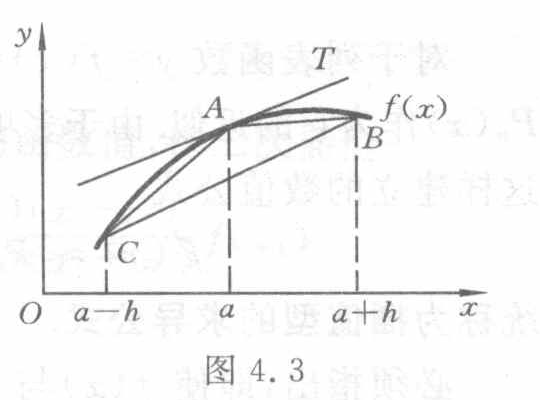
\includegraphics[width=0.85\linewidth,height=\textheight,keepaspectratio,alt={图 4.3（原书扫描裁切）}]{verified/assets/ch04b/figure-4-3.png}

图 4.3。原图标签：横轴 \(x\)、纵轴 \(y\)、原点 \(O\)；横轴位置 \(a-h\)、\(a\)、\(a+h\)，对应曲线上的点 \(C\)、\(A\)、\(B\)；曲线标记 \(f(x)\)，过 \(A\) 的切线标记 \(T\)。图中画出弦线 \(AB\)、\(AC\)、\(BC\) 与切线 \(AT\)。（此段为图中标签和图意的文字转录；原图未给出具体函数或数值。）

上述三种数值微分方法有个共同点，它们都是将导数的计算归结为计算 \(f\) 在若干节点上的函数值。这类数值微分方法称为机械求导方法。

要利用中点公式

\[
G(h)=\frac{f(a+h)-f(a-h)}{2h}
\]

计算导数 \(f'(a)\) 的近似值，首先必须选取合适的步长，为此需要进行误差分析。分别将 \(f(a\pm h)\) 在 \(x=a\) 处作 Taylor 展开，有

\[
f(a\pm h)=f(a)\pm hf'(a)+\frac{h^2}{2!}f''(a)
\pm\frac{h^3}{3!}f'''(a)+\frac{h^4}{4!}f^{(4)}(a)
\pm\frac{h^5}{5!}f^{(5)}(a)+\cdots,
\]

代入上式得

\[
G(h)=f'(a)+\frac{h^2}{3!}f'''(a)+\frac{h^4}{5!}f^{(5)}(a)+\cdots.
\]

\clearpage

原书 PDF 页 113；印刷页码 100。

\href{source-images/pdf-113.jpeg}{原页图像}

\subsubsection{4.5.1 中点方法（续）}\label{ch04b-ux4e2dux70b9ux65b9ux6cd5ux7eed}

由此得知，从截断误差的角度看，步长越小，计算结果越准确。

再考察舍入误差，按中点公式计算。当 \(h\) 很小时，因 \(f(a+h)\) 与 \(f(a-h)\) 很接近，直接相减会造成有效数字的严重损失（参见 1.4 节）。因此，从舍入误差的角度来看，步长是不宜太小的。

例如，用中点公式求 \(f(x)=\sqrt{x}\) 在 \(x=2\) 处的一阶导数，有

\[
G(h)=\frac{\sqrt{2+h}-\sqrt{2-h}}{2h}.
\]

设取四位数字计算，结果如表 4.6（导数的准确值 \(f'(2)=0.353\,553\)）所示。

\textbf{表 4.6}

{\def\LTcaptype{none} % do not increment counter
\begin{longtable}[]{@{}rrrrrr@{}}
\toprule\noalign{}
\(h\) & \(G(h)\) & \(h\) & \(G(h)\) & \(h\) & \(G(h)\) \\
\midrule\noalign{}
\endhead
\bottomrule\noalign{}
\endlastfoot
\(1\) & \(0.366\,0\) & \(0.05\) & \(0.353\,0\) & \(0.001\) & \(0.350\,0\) \\
\(0.5\) & \(0.356\,4\) & \(0.01\) & \(0.350\,0\) & \(0.000\,5\) & \(0.300\,0\) \\
\(0.1\) & \(0.353\,5\) & \(0.005\) & \(0.350\,0\) & \(0.000\,1\) & \(0.300\,0\) \\
\end{longtable}
}

在表 4.6 中，\(h=0.1\) 的逼近效果最好，如果进一步缩小步长，则逼近的效果会越来越差。

\subsubsection{4.5.2 插值型的求导公式}\label{ch04b-ux63d2ux503cux578bux7684ux6c42ux5bfcux516cux5f0f}

对于列表函数 \(y=f(x)\)（见表 4.7），运用插值原理，可以建立插值多项式 \(y=P_n(x)\) 作为它的近似。由于多项式的求导比较容易，取 \(P_n'(x)\) 的值作为 \(f'(x)\) 的近似值，这样建立的数值公式

\[
f'(x)\approx P_n'(x)
\tag{4.5.1}
\]

统称为插值型的求导公式。

\textbf{表 4.7}

{\def\LTcaptype{none} % do not increment counter
\begin{longtable}[]{@{}cccccc@{}}
\toprule\noalign{}
\(x\) & \(x_0\) & \(x_1\) & \(x_2\) & \(\cdots\) & \(x_n\) \\
\midrule\noalign{}
\endhead
\bottomrule\noalign{}
\endlastfoot
\(y\) & \(y_0\) & \(y_1\) & \(y_2\) & \(\cdots\) & \(y_n\) \\
\end{longtable}
}

必须指出，即使 \(f(x)\) 与 \(P_n(x)\) 的值相差不多，导数的近似值 \(P_n'(x)\) 与导数的真值 \(f'(x)\) 仍然可能差别很大，因而在使用求导公式（4.5.1）时应特别注意误差的分析。

依据插值余项定理，求导公式（4.5.1）的余项为

\[
f'(x)-P_n'(x)=\frac{f^{(n+1)}(\xi)}{(n+1)!}\omega_{n+1}'(x)
+\frac{\omega_{n+1}(x)}{(n+1)!}\frac{\mathrm{d}}{\mathrm{d}x}f^{(n+1)}(\xi),
\]

其中

\[
\omega_{n+1}(x)=\prod_{k=0}^{n}(x-x_i).
\]

在此余项公式中，由于 \(\xi\) 是 \(x\) 的未知函数，无法对其第二项 \(\dfrac{\omega_{n+1}(x)}{(n+1)!}\dfrac{\mathrm{d}}{\mathrm{d}x}f^{(n+1)}(\xi)\) 作出进一步的说明，因此，对于随意给出的点 \(x\)，误差 \(f'(x)-P_n'(x)\) 是无法预估的。但是，如果限定求某个节点 \(x_k\) 上的导数值，那么上面的第二项因 \(\omega_{n+1}(x_k)=0\) 而变为

（本句续下页。）

\begin{quote}
校注（agent 补充，CH04B-E004）：原页``其中''后的节点多项式印为 \(\prod_{k=0}^{n}(x-x_i)\)，乘积指标 \(k\) 与因子下标 \(i\) 不一致，已按原扫描保留。结合本页表 4.7 和下文 \(\omega_{n+1}(x_k)=0\)，应将因子写作 \((x-x_k)\)，或统一将乘积指标改为 \(i\)；这是原书疑似下标排印错误，非 OCR 错误。\href{verified/assets/ch04b/review-p113-product.png}{局部原扫描}。
\end{quote}

\clearpage

原书 PDF 页 114；印刷页码 101。

\href{source-images/pdf-114.jpeg}{原页图像}

\subsubsection{4.5.2 插值型的求导公式（续）}\label{ch04b-ux63d2ux503cux578bux7684ux6c42ux5bfcux516cux5f0fux7eed}

零，这时有余项公式

\[
f'(x_k)-P_n'(x_k)=\frac{f^{(n+1)}(\xi)}{(n+1)!}\omega_{n+1}'(x_k).
\tag{4.5.2}
\]

下面仅仅考察节点处的导数值。为简化讨论，假定所给的节点是等距的。

\paragraph{1. 两点公式}\label{ch04b-ux4e24ux70b9ux516cux5f0f}

设已给出两个节点 \(x_0,x_1\) 上面的函数值 \(f(x_0),f(x_1)\)，作线性插值公式

\[
P_1(x)=\frac{x-x_1}{x_0-x_1}f(x_0)+\frac{x-x_0}{x_1-x_0}f(x_1).
\]

对上式两端求导，记 \(x_1-x_0=h\)，有

\[
P_1'(x)=\frac1h[-f(x_0)+f(x_1)],
\]

于是有下列求导公式：

\[
P_1'(x_0)=\frac1h[f(x_1)-f(x_0)],\quad
P_1'(x_1)=\frac1h[f(x_1)-f(x_0)].
\]

而利用余项公式（4.5.2）知，带余项的两点公式是

\[
f'(x_0)=\frac1h[f(x_1)-f(x_0)]-\frac h2f''(\xi),
\]

\[
f'(x_1)=\frac1h[f(x_1)-f(x_0)]+\frac h2f''(\xi).
\]

\paragraph{2. 三点公式}\label{ch04b-ux4e09ux70b9ux516cux5f0f}

设已给出三个节点 \(x_0,x_1=x_0+h,x_2=x_0+2h\) 上的函数值，作二次插值

\[
\begin{aligned}
P_2(x)={}&\frac{(x-x_1)(x-x_2)}{(x_0-x_1)(x_0-x_2)}f(x_0)
+\frac{(x-x_0)(x-x_2)}{(x_1-x_0)(x_1-x_2)}f(x_1)\\
&+\frac{(x-x_0)(x-x_1)}{(x_2-x_0)(x_2-x_1)}f(x_2),
\end{aligned}
\]

令 \(x=x_0+th\)，上式可表示为

\[
P_2(x_0+th)=\frac12(t-1)(t-2)f(x_0)-t(t-2)f(x_1)
+\frac12t(t-1)f(x_2),
\]

两端对 \(t\) 求导，有

\[
P_2'(x_0+th)=\frac1{2h}[(2t-3)f(x_0)-(4t-4)f(x_1)+(2t-1)f(x_2)].
\tag{4.5.3}
\]

这里撇号表示对变量 \(x\) 求导数。上式分别取 \(t=0,1,2\)，得到以下三种三点公式：

\[
P_2'(x_0)=\frac1{2h}[-3f(x_0)+4f(x_1)-f(x_2)],
\]

\[
P_2'(x_1)=\frac1{2h}[-f(x_0)+f(x_2)],
\]

（第三个公式续下页。）

\clearpage

原书 PDF 页 115；印刷页码 102。

\href{source-images/pdf-115.jpeg}{原页图像}

\subsubsection{4.5.2 插值型的求导公式（续）}\label{ch04b-ux63d2ux503cux578bux7684ux6c42ux5bfcux516cux5f0fux7eed-1}

\paragraph{2. 三点公式（续）}\label{ch04b-ux4e09ux70b9ux516cux5f0fux7eed}

\[
P_2'(x_2)=\frac1{2h}[f(x_0)-4f(x_1)+3f(x_2)],
\]

而带余项的三点求导公式为

\[
f'(x_0)=\frac1{2h}[-3f(x_0)+4f(x_1)-f(x_2)]+\frac{h^2}3f'''(\xi),
\]

\[
f'(x_1)=\frac1{2h}[-f(x_0)+f(x_2)]-\frac{h^2}6f'''(\xi),
\tag{4.5.4}
\]

\[
f'(x_2)=\frac1{2h}[f(x_0)-4f(x_1)+3f(x_2)]+\frac{h^2}3f'''(\xi),
\]

其中式（4.5.4）是我们所熟悉的中点公式。在三点公式中，它由于少用了一个函数值 \(f(x_1)\) 而引人注目。

用插值多项式 \(P_n(x)\) 作为 \(f(x)\) 的近似函数，还可以建立高阶数值微分公式

\[
f^{(k)}(x)\approx P_n^{(k)}(x),\quad k=1,2,\cdots.
\]

例如，将式（4.5.3）再对 \(t\) 求导一次，有

\[
P_2''(x_0+th)=\frac1{h^2}[f(x_0)-2f(x_1)+f(x_2)],
\]

于是有

\[
P_2''(x_1)=\frac1{h^2}[f(x_1-h)-2f(x_1)+f(x_1+h)],
\]

而带余项的二阶三点公式为

\[
f''(x_1)=\frac1{h^2}[f(x_1-h)-2f(x_1)+f(x_1+h)]-\frac{h^2}{12}f^{(4)}(\xi).
\tag{4.5.5}
\]

\subsubsection{4.5.3 实用的五点公式}\label{ch04b-ux5b9eux7528ux7684ux4e94ux70b9ux516cux5f0f}

设已给出五个节点 \(x_i=x_0+ih,\quad i=0,1,2,3,4\) 上的函数值，重复同样的手续，不难导出下列五点公式：

\[
m_0=\frac1{12h}[-25f(x_0)+48f(x_1)-36f(x_2)+16f(x_3)-3f(x_4)],
\]

\[
m_1=\frac1{12h}[-3f(x_0)-10f(x_1)+18f(x_2)-6f(x_3)+f(x_4)],
\]

\[
m_2=\frac1{12h}[f(x_0)-8f(x_1)+8f(x_3)-f(x_4)],
\]

\[
m_3=\frac1{12h}[-f(x_0)+6f(x_1)-18f(x_2)+10f(x_3)+3f(x_4)],
\]

\[
m_4=\frac1{12h}[3f(x_0)-16f(x_1)+36f(x_2)-48f(x_3)+25f(x_4)].
\]

其中 \(m_i\) 代表一阶导数 \(f'(x_i)\) 的近似值，读者不难导出这些求导公式的余项。

再记 \(M_i\) 表示二阶导数 \(f''(x_i)\) 的近似值，二阶五点公式如下：

（公式续下页。）

\clearpage

原书 PDF 页 116；印刷页码 103。

\href{source-images/pdf-116.jpeg}{原页图像}

\subsubsection{4.5.3 实用的五点公式（续）}\label{ch04b-ux5b9eux7528ux7684ux4e94ux70b9ux516cux5f0fux7eed}

\[
M_0=\frac1{12h^2}[35f(x_0)-104f(x_1)+114f(x_2)-56f(x_3)+11f(x_4)],
\]

\[
M_1=\frac1{12h^2}[11f(x_0)-20f(x_1)+6f(x_2)+4f(x_3)-f(x_4)],
\]

\[
M_2=\frac1{12h^2}[-f(x_0)+16f(x_1)-30f(x_2)+16f(x_3)-f(x_4)],
\]

\[
M_3=\frac1{12h^2}[-f(x_0)+4f(x_1)+6f(x_2)-20f(x_3)+11f(x_4)],
\]

\[
M_4=\frac1{12h^2}[11f(x_0)-56f(x_1)+114f(x_2)-104f(x_3)+35f(x_4)].
\]

对于给定的一张数据表，用五点公式求节点上的导数值往往可以获得满意的结果。五个相邻节点的选择原则，一般是在所考察的节点的两侧各取两个邻近的节点，如果一侧的节点数不足两个（即一侧只有一个节点或没有节点），则用另一侧的节点补足。

\textbf{例 4.4}　利用 \(f(x)=\sqrt{x}\) 的一张数据表，按五点公式求节点上的导数值 \(m_i\) 与 \(M_i\)，并与导数的准确值比较，如表 4.8 所示。

\textbf{表 4.8}

{\def\LTcaptype{none} % do not increment counter
\begin{longtable}[]{@{}
  >{\raggedleft\arraybackslash}p{(\linewidth - 10\tabcolsep) * \real{0.1667}}
  >{\raggedleft\arraybackslash}p{(\linewidth - 10\tabcolsep) * \real{0.1667}}
  >{\raggedleft\arraybackslash}p{(\linewidth - 10\tabcolsep) * \real{0.1667}}
  >{\raggedleft\arraybackslash}p{(\linewidth - 10\tabcolsep) * \real{0.1667}}
  >{\raggedleft\arraybackslash}p{(\linewidth - 10\tabcolsep) * \real{0.1667}}
  >{\raggedleft\arraybackslash}p{(\linewidth - 10\tabcolsep) * \real{0.1667}}@{}}
\toprule\noalign{}
\begin{minipage}[b]{\linewidth}\raggedleft
\(x_i\)
\end{minipage} & \begin{minipage}[b]{\linewidth}\raggedleft
\(f(x_i)\)
\end{minipage} & \begin{minipage}[b]{\linewidth}\raggedleft
\(m_i\)
\end{minipage} & \begin{minipage}[b]{\linewidth}\raggedleft
\(f'(x_i)\)
\end{minipage} & \begin{minipage}[b]{\linewidth}\raggedleft
\(M_i/\times10^3\)
\end{minipage} & \begin{minipage}[b]{\linewidth}\raggedleft
\(f''(x_i)/\times10^3\)
\end{minipage} \\
\midrule\noalign{}
\endhead
\bottomrule\noalign{}
\endlastfoot
\(100\) & \(10.000\,000\) & \(0.050\,000\) & \(0.050\,000\) & \(-0.247\,58\) & \(-0.250\,00\) \\
\(101\) & \(10.049\,875\) & \(0.049\,751\) & \(0.049\,752\) & \(-0.245\,91\) & \(-0.246\,30\) \\
\(102\) & \(10.099\,504\) & \(0.049\,507\) & \(0.049\,507\) & \(-0.241\,91\) & \(-0.242\,68\) \\
\(103\) & \(10.148\,891\) & \(0.049\,267\) & \(0.049\,266\) & \(-0.239\,58\) & \(-0.239\,16\) \\
\(104\) & \(10.198\,039\) & \(0.049\,029\) & \(0.049\,029\) & \(-0.236\,91\) & \(-0.235\,72\) \\
\(105\) & \(10.246\,950\) & \(0.048\,795\) & \(0.048\,795\) & \(-0.236\,66\) & \(-0.232\,36\) \\
\end{longtable}
}

\subsubsection{4.5.4 样条求导}\label{ch04b-ux6837ux6761ux6c42ux5bfc}

我们知道，样条函数 \(S(x)\) 作为 \(f(x)\) 的近似函数，不但彼此的函数值很接近，导数值也很接近。例如，对于三次样条 \(S_3(x)\)，有

\[
|f^{(a)}(x)-S_3^{(a)}(x)|=O(h^{4-a})\qquad(a=0,1,2,3),
\]

因此，用样条函数建立数值微分公式是很自然的，即

\[
f^{(a)}(x)\approx S_3^{(a)}(x)\qquad(a=0,1,2,3).
\tag{4.5.6}
\]

与前述插值型微分公式（4.5.1）不同，样条微分公式（4.5.6）可以用来计算插值范围内任何一点 \(x\)（不仅是节点 \(x_i\)）上的导数值。对于等距分划

\[
\pi:a=x_0<x_1<x_2<\cdots<x_n=b,\quad x_{k+1}-x_k=h,
\]

三次样条 \(S_3(x)\) 在节点上的导数值 \(S_3'(x_k)=m_k\) 满足下列连续性方程组

（方程组续下页。）

\begin{quote}
校注（agent 补充，原表记法说明）：表 4.8 后两列表头按原扫描保留为 \(M_i/\times10^3\) 与 \(f''(x_i)/\times10^3\)，未改写原表头。表内数值对应导数乘 \(10^3\) 后的数值，例如 \(f''(100)=-1/(4\cdot100^{3/2})=-0.00025\)，表中列为 \(-0.25000\)；此说明仅解释该页缩放记法。\href{verified/assets/ch04b/review-table-4-8.png}{表 4.8 原扫描局部}。
\end{quote}

\clearpage

原书 PDF 页 117；印刷页码 104。

\href{source-images/pdf-117.jpeg}{原页图像}

\subsubsection{4.5.4 样条求导（续）}\label{ch04b-ux6837ux6761ux6c42ux5bfcux7eed}

\[
m_{k-1}+4m_k+m_{k+1}=3(y_{k+1}-y_{k-1})/h,\quad k=1,2,\cdots,n-1.
\tag{4.5.7}
\]

设已给出端点处的一阶导数值 \(m_0=y_0',m_n=y_n'\)，则求解方程组（4.5.7）得出的 \(m_k\) 即可作为导数 \(f'(x_k)\) 的近似值。

\subsection{小结}\label{ch04b-ux5c0fux7ed3}

本章介绍积分和微分的数值计算方法。我们知道，积分和微分是两种分析运算，它们都是用极限来定义的。数值积分和数值微分则归结为函数值的四则运算，从而使计算过程可以在计算机上完成。

处理数值积分和数值微分的基本方法是逼近法：设法构造某个简单函数 \(P(x)\) 近似 \(f(x)\)，然后对 \(P(x)\) 求积（求导）得到 \(f(x)\) 的积分（导数）的近似值。本章基于插值原理推导了数值积分和数值微分的基本公式。

插值求积公式分 Newton-Cotes 公式与 Gauss 公式两类。前者取等距节点，算法简单而容易编制程序。Gauss 公式的精度高，但节点没有规律。运用带权的 Gauss 公式，能把复杂的积分化简，还可以直接计算奇异积分。构造 Gauss 公式会碰到选取求积节点（所谓 Gauss 点）的困难。

梯形法是众所周知的一种简单的求积方法。可以看到，将二分过程中的梯形值适当进行加权平均，会获得高精度的积分值。运用这种外推加速技术的 Romberg 算法，在电子计算机上有着广泛的应用。

限于篇幅，本章略去了数值积分的一些重要内容，如奇异积分、振荡函数的积分等，这些内容在文献 {[}7{]} 中有较为详尽的论述。关于高维积分的数值计算，有兴趣的读者可参看文献 {[}8{]}。

\subsection{习题}\label{ch04b-ux4e60ux9898}

\textbf{1.} 确定下列求积公式中的待定参数，使其代数精度尽量高，并指明所构造出的求积公式所具有的代数精度：

（1）

\[
\int_{-h}^{h}f(x)\,\mathrm{d}x\approx A_{-1}f(-h)+A_0f(0)+A_1f(h);
\]

（2）

\[
\int_{-2h}^{2h}f(x)\,\mathrm{d}x\approx A_{-1}f(-h)+A_0f(0)+A_1f(h);
\]

（3）

\[
\int_{-1}^{1}f(x)\,\mathrm{d}x\approx[f(-1)+2f(x_1)+3f(x_2)]/3;
\]

（4）

\[
\int_0^h f(x)\,\mathrm{d}x\approx h[f(0)+f(h)]/1+ah^2[f'(0)-f'(h)].
\]

\textbf{2.} 分别用梯形公式和 Simpson 公式计算下列积分：

（1）

\[
\int_0^1\frac{x}{4+x^2}\,\mathrm{d}x,\quad n=8;
\]

（2）

\[
\int_0^1\frac{(1-e^{-x})^{\frac12}}{x}\,\mathrm{d}x,\quad n=10;
\]

（第 2 题其余小题续下页。）

\begin{quote}
校注（agent 补充，CH04B-E005）：第 1 题（4）首项的分母在原扫描中明确印为``1''，故保留 \(h[f(0)+f(h)]/1\)。该处疑为原书排印错误：仅作排印一致性检查，当 \(f\equiv1\) 时，积分为 \(h\)，而所印右端为 \(2h\)，并且导数项为零；疑应将分母印为``2''。此处不求解题中参数或代数精度。\href{verified/assets/ch04b/review-p117-exercises.png}{习题原扫描局部}。
\end{quote}

\clearpage

原书 PDF 页 118；印刷页码 105。

\href{source-images/pdf-118.jpeg}{原页图像}

\subsection{习题（续）}\label{ch04b-ux4e60ux9898ux7eed}

\textbf{2.（续）}

（3）

\[
\int_1^9\sqrt{x}\,\mathrm{d}x,\quad n=4;
\]

（4）

\[
\int_0^{\pi/6}\sqrt{4-\sin^2\varphi}\,\mathrm{d}\varphi,\quad n=6.
\]

\textbf{3.} 直接验证 Cotes 公式（4.2.4）具有五次代数精度。

\textbf{4.} 用 Simpson 公式求积分 \(\displaystyle\int_0^1 e^{-x}\,\mathrm{d}x\) 并估计误差。

\textbf{5.} 推导下列三种矩形求积公式：

\[
\int_a^b f(x)\,\mathrm{d}x=(b-a)f(a)+\frac{f'(\eta)}2(b-a)^2,
\]

\[
\int_a^b f(x)\,\mathrm{d}x=(b-a)f(b)-\frac{f'(\eta)}2(b-a)^2,
\]

\[
\int_a^b f(x)\,\mathrm{d}x=(b-a)f\left(\frac{a+b}2\right)+\frac{f''(\eta)}{24}(b-a)^3.
\]

\textbf{6.} 证明梯形公式（4.2.9）和 Simpson 公式（4.2.11）当 \(n\to\infty\) 时收敛到积分 \(\displaystyle\int_a^b f(x)\,\mathrm{d}x\)。

\textbf{7.} 用复化梯形公式求积分 \(\displaystyle\int_a^b f(x)\,\mathrm{d}x\)。要将积分区间 \([a,b]\) 分成多少等份，才能保证误差不超过 \(\varepsilon\)（不计舍入误差）？

\textbf{8.} 用 Romberg 方法计算积分 \(\displaystyle\frac2{\sqrt\pi}\int_0^1 e^{-x}\,\mathrm{d}x\)，要求误差不超过 \(10^{-5}\)。

\textbf{9.} 卫星轨道是一个椭圆，椭圆周长的计算公式是

\[
s=a\int_0^{\pi/2}\sqrt{1-\left(\frac ca\right)^2\sin^2\theta}\,\mathrm{d}\theta,
\]

其中 \(a\) 是椭圆的长半轴，\(c\) 是地球中心与轨道中心（椭圆中心）的距离。记 \(h\) 为近地点距离，\(H\) 为远地点距离，\(R=6\,371\ \mathrm{km}\) 为地球半径，则 \(a=(2R+H+h)/2,\quad c=(H-h)/2\)。

我国第一颗人造卫星近地点距离 \(h=439\ \mathrm{km}\)，远地点距离 \(2\,384\ \mathrm{km}\)，试求卫星轨道的周长。

\textbf{10.} 证明等式

\[
n\sin\frac\pi n=\pi-\frac{\pi^3}{3!\,n^2}+\frac{\pi^5}{5!\,n^4}-\cdots,
\]

试依据 \(n\sin\dfrac\pi n\)（\(n=3,6,12\)）的值，用外推算法求 \(\pi\) 的近似值。

\textbf{11.} 用下列方法计算积分 \(\displaystyle\int_1^3\frac{\mathrm{d}y}{y}\)，并比较结果。

（1）Romberg 方法；

（2）三点及五点 Gauss 公式；

（3）将积分区间分为四等份，用复化两点 Gauss 公式。

\textbf{12.} 用三点公式和五点公式求 \(f(x)=\dfrac1{(1+x)^2}\) 在 \(x=1.0,1.1\) 和 \(1.2\) 处的导数值，并估计误差。\(f(x)\) 的值由表 4.9 给出。

\textbf{表 4.9}

{\def\LTcaptype{none} % do not increment counter
\begin{longtable}[]{@{}
  >{\centering\arraybackslash}p{(\linewidth - 10\tabcolsep) * \real{0.1667}}
  >{\centering\arraybackslash}p{(\linewidth - 10\tabcolsep) * \real{0.1667}}
  >{\centering\arraybackslash}p{(\linewidth - 10\tabcolsep) * \real{0.1667}}
  >{\centering\arraybackslash}p{(\linewidth - 10\tabcolsep) * \real{0.1667}}
  >{\centering\arraybackslash}p{(\linewidth - 10\tabcolsep) * \real{0.1667}}
  >{\centering\arraybackslash}p{(\linewidth - 10\tabcolsep) * \real{0.1667}}@{}}
\toprule\noalign{}
\begin{minipage}[b]{\linewidth}\centering
\(x\)
\end{minipage} & \begin{minipage}[b]{\linewidth}\centering
\(1.0\)
\end{minipage} & \begin{minipage}[b]{\linewidth}\centering
\(1.1\)
\end{minipage} & \begin{minipage}[b]{\linewidth}\centering
\(1.2\)
\end{minipage} & \begin{minipage}[b]{\linewidth}\centering
\(1.3\)
\end{minipage} & \begin{minipage}[b]{\linewidth}\centering
\(1.4\)
\end{minipage} \\
\midrule\noalign{}
\endhead
\bottomrule\noalign{}
\endlastfoot
\(f(x)\) & \(0.250\,0\) & \(0.226\,8\) & \(0.206\,6\) & \(0.189\,0\) & \(0.173\,6\) \\
\end{longtable}
}

\begin{quote}
校注（agent 补充，CH04B-E006）：第 9 题的原扫描明确写 \(s=a\int_0^{\pi/2}\cdots\,\mathrm{d}\theta\)，本转录保留原式。若 \(s\) 表示文中的椭圆``周长''，该式疑漏系数 \(4\)：所印表达式对应四分之一周长；以 \(c=0\) 的圆作一致性检查，原式给出 \(\pi a/2\)，而圆周长为 \(2\pi a\)。仅记录原书公式疑误，不代做本题数值计算。\href{verified/assets/ch04b/review-p118-orbit.png}{局部原扫描}。
\end{quote}

